During the second year of project activities integration activities
started. In the integration process, the architecture initially
presented in Deliverable D8.1 was deeply revised. This process was
required in order to align the activities carried out within the
project's technical work packages (WP2-WP7) and to ensure
interoperability among the components developed by the various
partners. In this section we briefly present the architecture as it
currently stands (at M24). No major changes are currently foreseen,
even if ---given the research-oriented nature of the SmartSociety
project--- this cannot be guaranteed. In this sense, the architectural
specifications of the SmartSociety platform have to be seen as a live document, which reflects the
actual progress of the research activities carried out by Consortium
partners. 

\subsection{Logical View}


The logical view of the SmartSociety platform is presented in Fig.~\ref{fig:logical_view}. The Consortium has identified 9 key
components which jointly provide the required functionality:

\begin{figure}[!hbt]
 \centering
 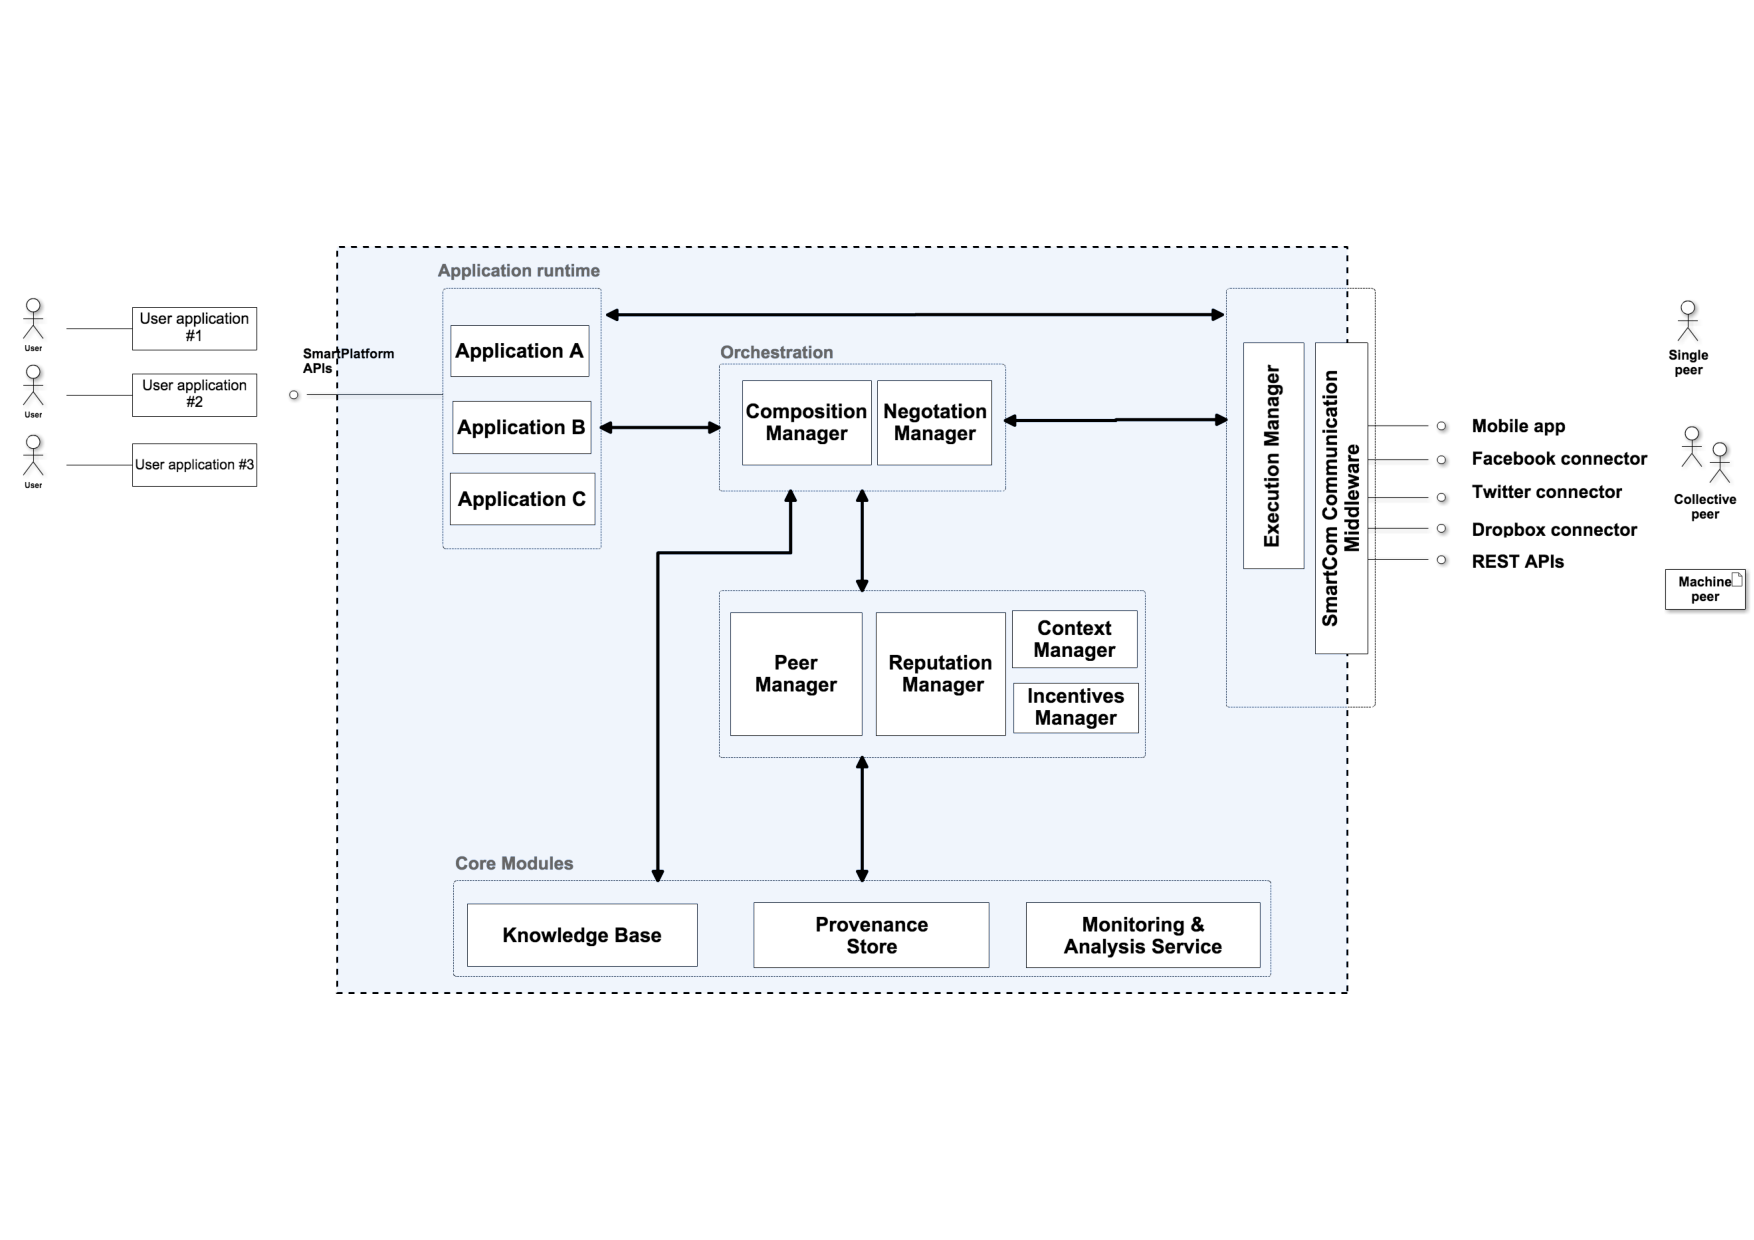
\includegraphics[width=0.7\textwidth, angle = -90]{figs/logical_view.pdf}
 \caption{SmartSociety logical view.}
 \label{fig:logical_view}
\end{figure}

The core components which are part of the revised version of the SmartSociety are the following:
\begin{itemize}
\item \textbf{Application Runtime}: the application runtime is the component where the applications created by developers will run. The runtime provides all the necessary programming abstractions for interacting with the various internal components provided by the SmartSociety platform. 

\item \textbf{Orchestration}: it provides two key functionalities: composition and negotiaton. Composition takes as
inputs tasks and interacts with the peer manager to find suitable peers for completing the task. The negotiation manager is in charge of handling the negotiation process with peers in order to ensure that
the necessary services and resources required to carry out the task the orchestration is in charge of the complete orchestration of a given computation task. This includes the initial creation of a \textit{composition} which can fulfill a given computation task, whereas a composition determines (i) the peers which can potentially execute such task, and (ii) the necessary interactions and/or external services which are needed to execute such task. 

\item \textbf{Peer Manager}: the Peer Manager is the module responsible for managing all peers-related information. This includes their profile, as well as any other information which will then be used by the Orchestration component for identifying possible peers which can execute a certain task.  It maintains a profile of each peer, which
represents a model thereof in terms of knowledge, resources and
capacity. It provides a peer search functionality that allows other
components to find for the most appropriate peers for a given tasks.  Besides individual peers, the PeerManager also manages collectives, which are groups of peers characterized by specific properties (see Deliverable XXX for additional details on collectives).

\item \textbf{Reputation Manager}: the Reputation Manager handles the reputation of peers. It computes the
reputation of a given peer based on feedback from users. It uses data from the provenance store in order to carry out the computatio Reputation is based on various metrics that the system will be able to compute, starting from peers' execution of tasks. A reputation score will be computed for every single peer, and this information will be available to the Peer Manager when selecting peers for the execution of tasks.

\item \textbf{Knowledge Base}: the Knowledge Base (KB) is shared among the various components of the platform, and contains an agreed ontology about peers, task, workflows, incentives, etc.. It provides the domain terminology, as well as all the semantic relations between terms. In particular, the knowledge base is responsible for ensuring that all component share a common understanding of the inputs/outputs between any two parties of the platform.
The overall knowledge base will be divided into domains, which allow to capture the diversity of the entities being part of SmartSociety. A semantic reasoner will allow to perform semantic queries over the knowledge base.

\item \textbf{Provenance Store}: it logs actions performed by platform
components and peers according to the W3C PROV recommendation. In particular, the provenance store is the component responsible for keeping track of how the overall compositions are being created, executed and how the data managed by the platform is being transformed. It will play a fundamental role in the evaluation of peers reputation, as well as in ensuring that the system as a whole enforces the proper privacy constraints imposed by the peers.It further supports an auditing service which is able to reconstruct and visualize provenance trails. 
\item \textbf{Execution Manager}: the execution manager deals with the different interaction patterns that might be required to interact with peers.
\item Monitoring and analytics service: this service logs and monitors
the platform jobs and can be used by platform administrators to
perform root-cause analysis and to extract analytics on the
performance of the system. 
\item Elasticity manager:

\item Incentives manager: it provides insight on incentives and
interventions that can be used to achieve higher quality results.
\end{itemize} 	


\subsection{Deployment View and Network Diagrams}
The SmartSociety platform has been designed around a REST architecture
with the aim of supporting flexibility in the deployment model. This
means that the platform shall seamlessly support both single-tenant as
well as multi-tenant deployment models. Also, the platform component
can be centralised on a single infrastructure or can be distributed
across different servers. The choice of the specific deployment model
to be used depends on technical as well as business considerations. In
the remainder of this section we present, as a use case, the current
deployment utilised for integration, testing, validation and
experimentation purposes. This is by no means to be considered the
only model supported, but it provides an actual example of the
supported configuration. 

\subsection{Dynamic View}
Fig.~\ref{fig:dynamic_view} provide the dynamic view of how the various components of the SmartSociety platform interact with each other, when running an application based on SmartSociety. 

\begin{figure}[!hbt]
 \centering
 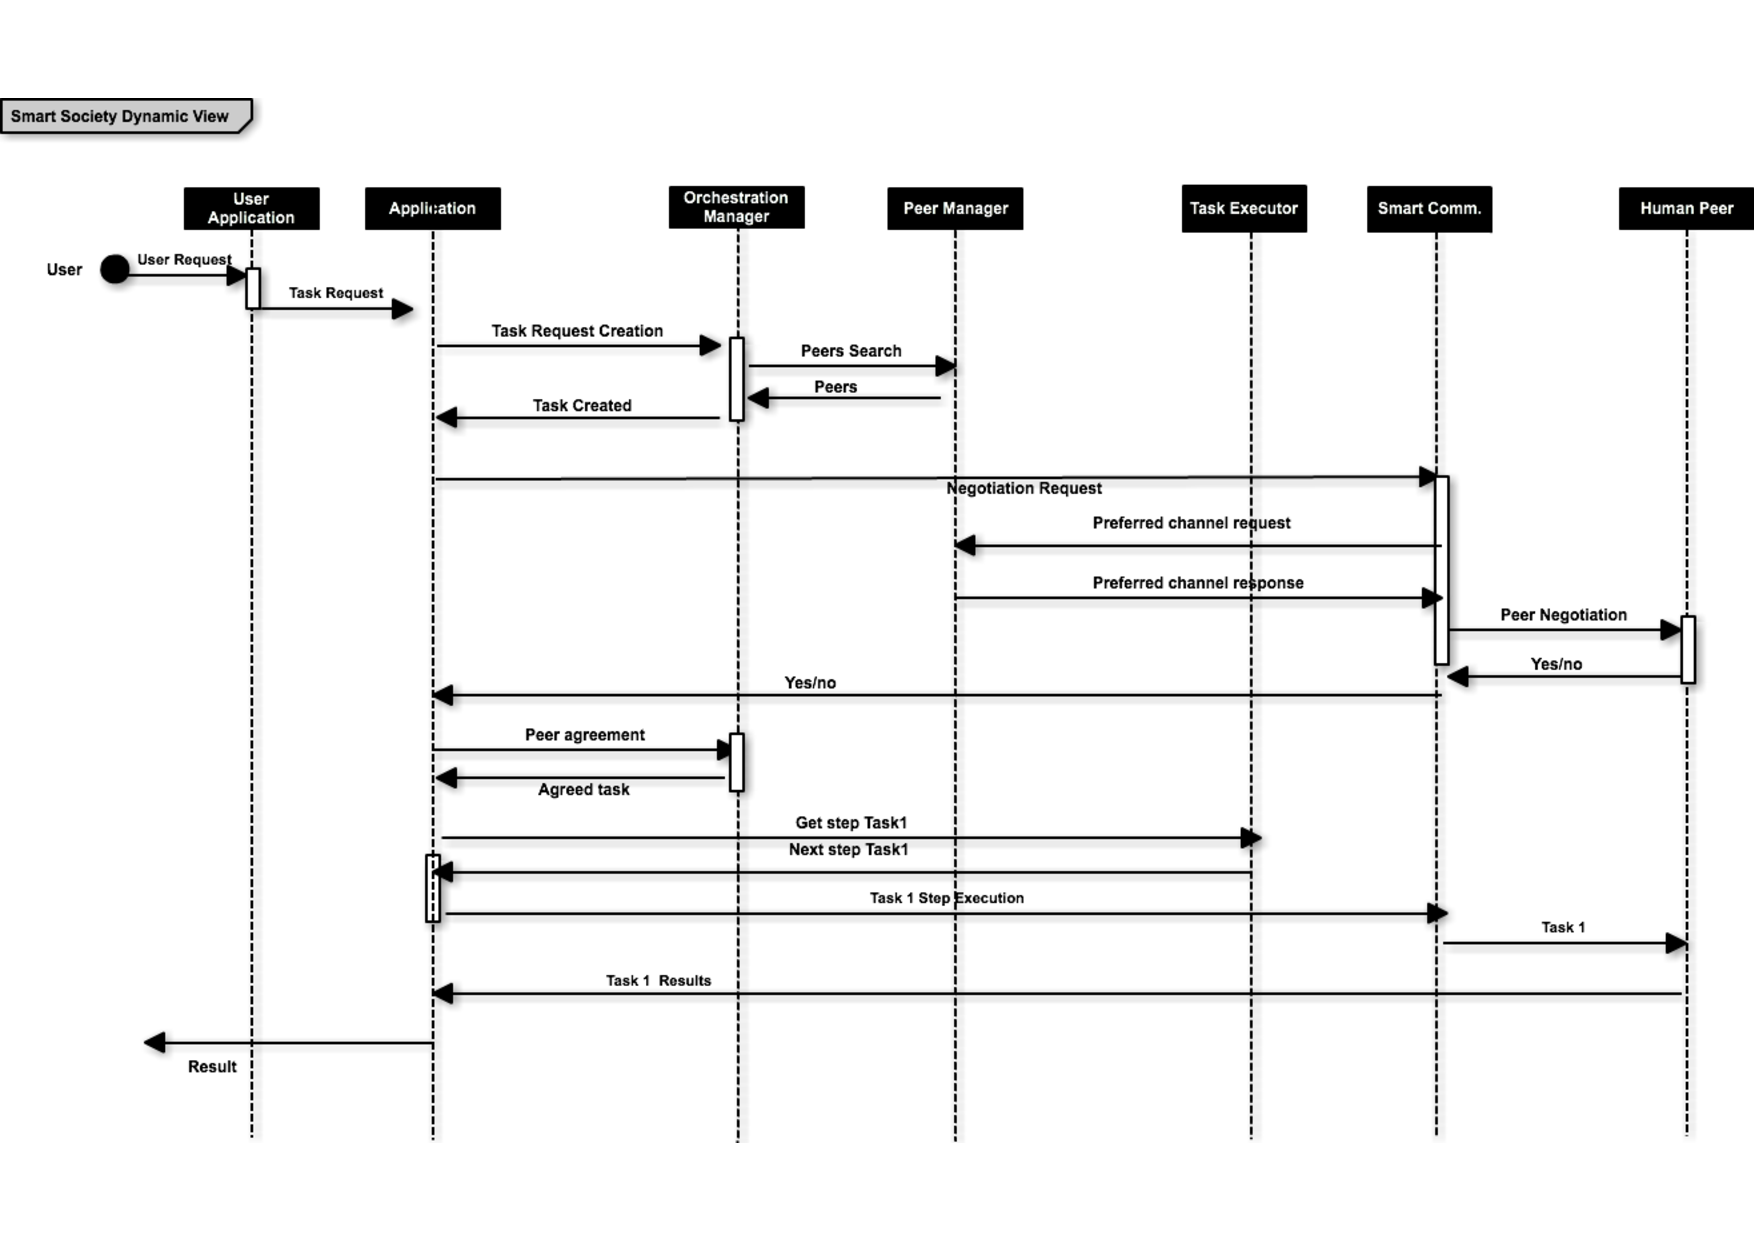
\includegraphics[width=1\textwidth]{figs/dynamic_view.pdf}
 \caption{SmartSociety dynamic view.}
 \label{fig:dynamic_view}
\end{figure}

The sequence diagram can be summarized in the following steps:
\begin{itemize}
\item platform invocation: the starting point is a user application (e.g., a mobile application) which is exploiting the SmartSociety platform for running a human computation task (refer to Sec.~\ref{sec:asksmartsoc} for a more concrete example). The request is directed towards an application deployed in the SmartSociety application and providing the necessary support for executing the requested task. The invocation will contain all the necessary metadata for fully describing the task, according to the APIs offered by the application running in the platform.
\item composition request: the application, after receiving the request from the user application, converts it into a \textit{composition job request}. A composition is the request to create a composition of peers/collectives capable of executing the task. The composition job request happens through the programming abstractions provided by the runtime, which allow to fully characterize the task that needs to be executed.
\item   
\end{itemize}


The SmartSociety platform is meant to support a rather wide range of
social computation patterns (or templates). In order to provide
insight into the flexibility of the platform and the actual
interworking of components, we have developed sequence diagrams for two
'extreme' applications:
\begin{itemize}
\item SmartShare is a ridesharing system able to account for user's
preferences and to compute recommendations based on the feedback
provided by other service users. It is what we call a 'full
negotiation' scenario, in which the computational task of finding an
agreement on the rides is left to individuals and collectives. The
platform in this case is used to carry out administration tasks, in
particular keeping track of the rides and ride requests, their status
and to maintain reputation of drivers and passengers.
\item AskSmartSociety! is a Q\&A service supporting hybridity. The
computational pattern here is that typical of micro-tasking
applications (\'a la Mechanical Turk, roughly speaking), where the
task in this corresponds to a question to be answered. The service
supports hybrid computation in that questions can be transparently
provided by machine peers or human peers. Quality criteria can be
specified in order to define when a chosen answer has to be presented
to the user. 
\end{itemize}
In the following we present details about the two aforementioned
applications. 
\subsubsection{Example: SmartShare}
\begin{figure}
\centering
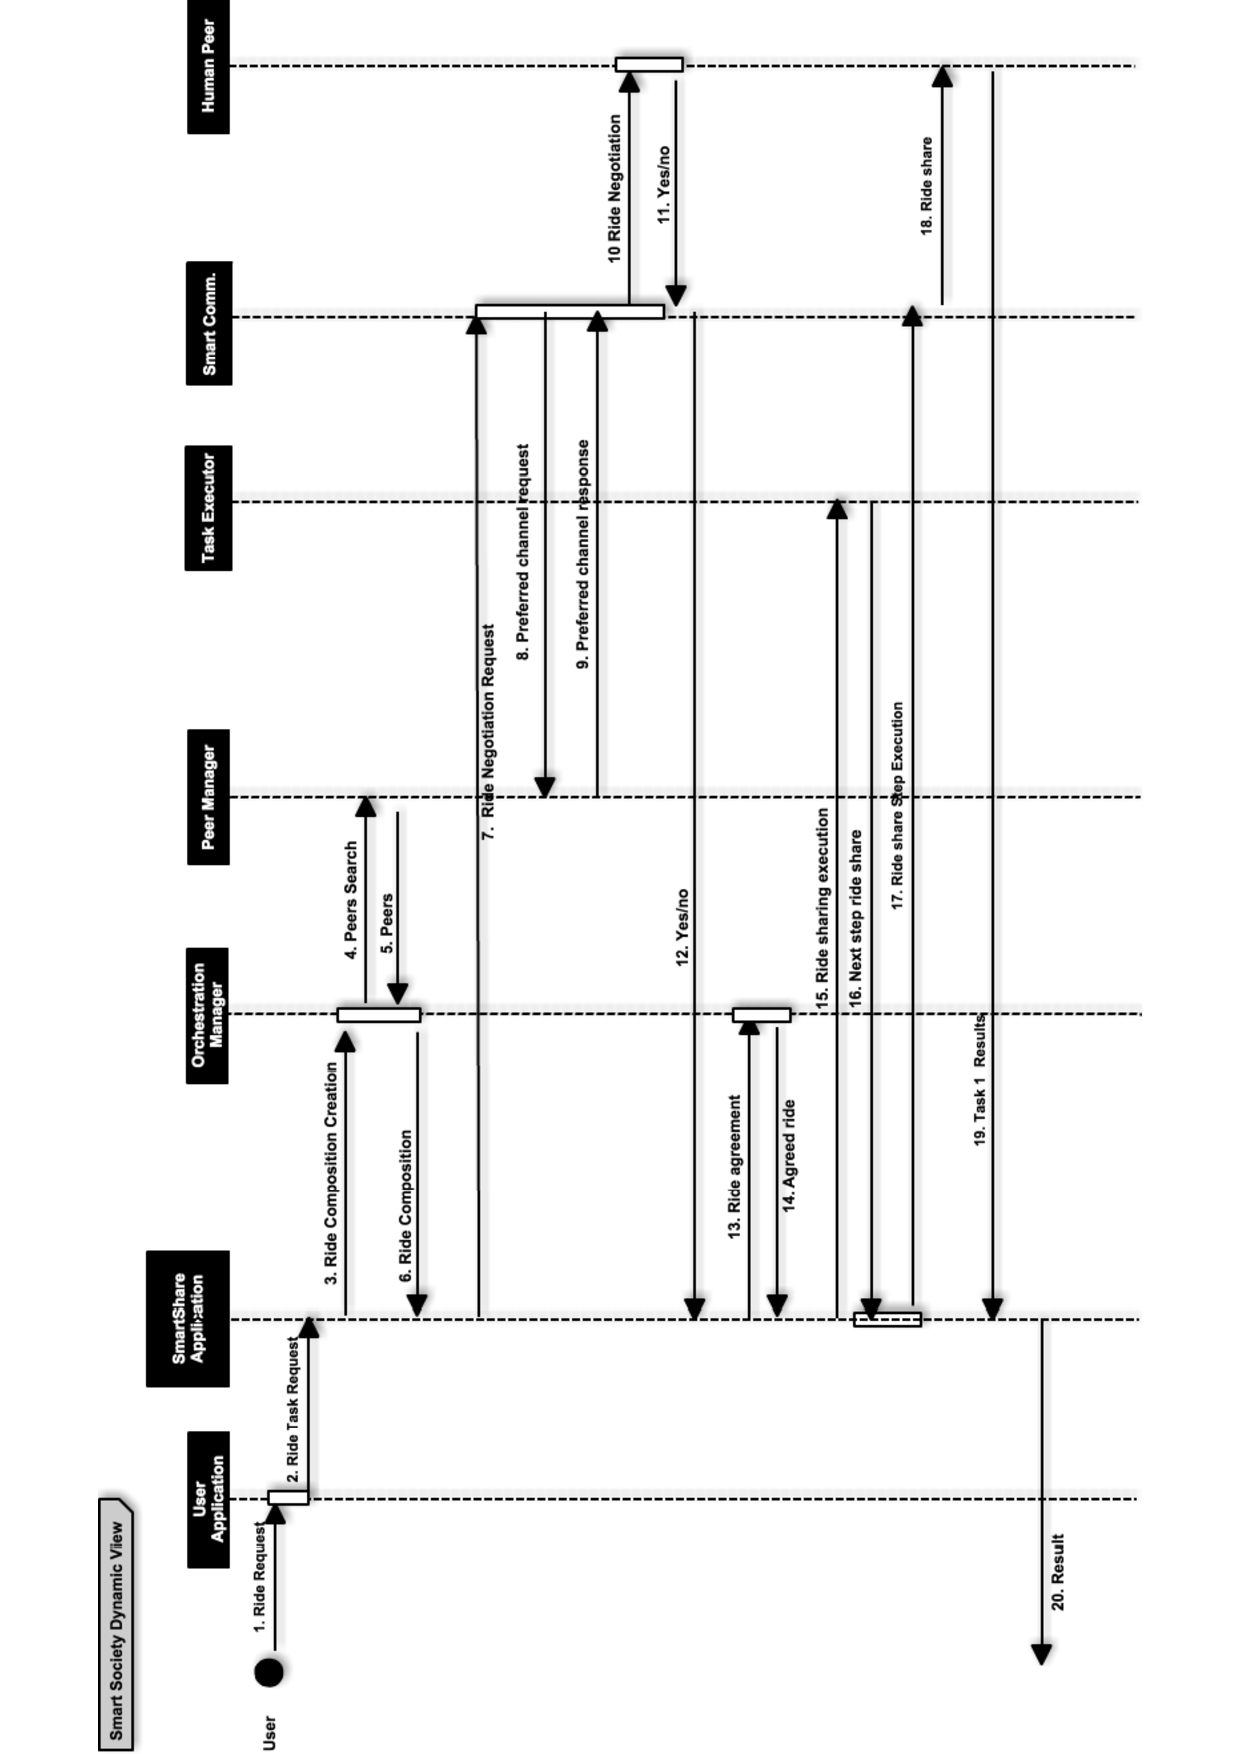
\includegraphics[width=0.9\textwidth]{./figs/sequenceRide}
\caption{Sequence diagram of the SmartShare application.}
\label{fig:dynamic_share}
\end{figure}

\subsection{Example: Ask SmartSociety}\label{sec:asksmartsoc}
\textit{Ask SmartSociety} is a simple Questions and Answer service enabled by the SmartSociety platform which has been used as the benchamark for implementing the initial version of the SmartSociety platform. It focus on tourism, which is the reference domain to be used for validating the SmartSociety vision.\\
Ask SmartSociety! will be a service where users can post questions in natural languages and peers can provide answers. Peers providing answers can be humans (individuals or collectives) as well as machines (intelligent software agents). Peers can compose (forming collectives, hybrid or not) to provide answers. Answers can be ranked based on the reputation of the peers or on community ranking (similarly to stackoverflow). In some instances the user issuing the question can select an answer and provide feedback on the peer providing it.
Two examples (grounded in the tourism application scenarios) can help in understanding the features of the Ask SmartSociety! service:

\textit{Next week Peter will fly to Venice. He will be busy in meetings during the day but wants to explore some ‘hidden’ places at night. He could well explore various online tourist sites but he prefers to ask experts and local people. He could also google for relevant content, but he does not actually need an answer right away, he just needs to get it in one week. And having one system which allows him to query local experts, web-based recommendation services and incoming tourism institutions looks definitely appealing to him!
Alice is visiting Milano during the next week. It is his first time in Milan, and she is looking for a restaurant in the city centre. Since it is spring time, she would love eat outside and therefore  find a restaurant with a garden. Alice is also celiac, and she needs to find restaurants, which do have gluten free menus. She relies on the Ask SmartSociety! application for retrieving some suggestions on where to have dinner during her stay in Milan. She is looking for unconventional recommendations.}


\begin{figure}
\centering
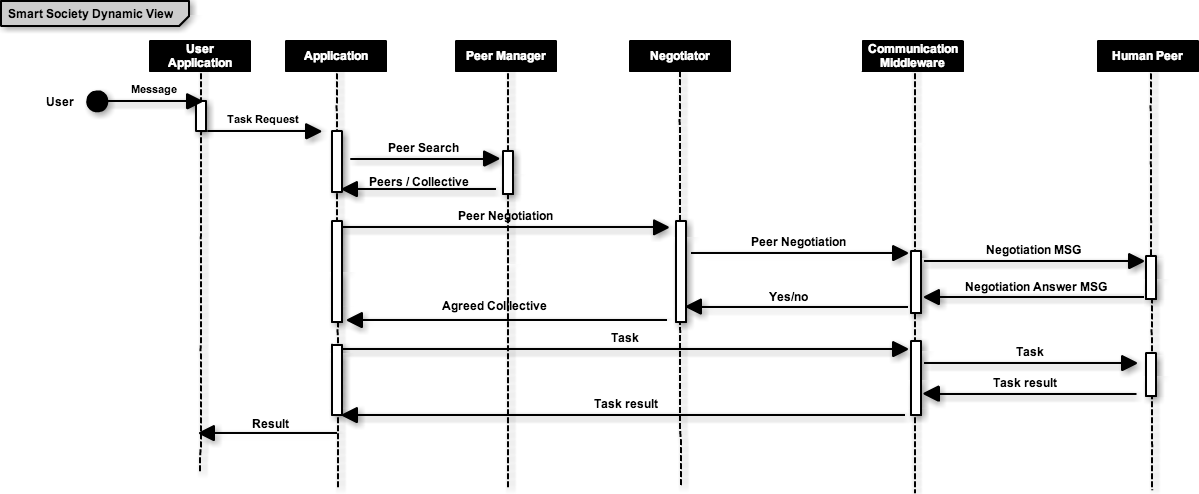
\includegraphics[width=0.9\textwidth]{./figs/sequenceAsk}
\caption{Sequence diagram for AskSmartSociety! applications.}
\label{fig:dynamic_ask}
\end{figure}